\documentclass[
  12pt,
  bibliography=totoc,     % Literatur im Inhaltsverzeichnis
  captions=tableheading,  % Tabellenüberschriften
  titlepage=firstiscover, % Titelseite ist Deckblatt
]{scrartcl}

% Paket float verbessern
\usepackage{scrhack}

% Warnung, falls nochmal kompiliert werden muss
\usepackage[aux]{rerunfilecheck}

% unverzichtbare Mathe-Befehle
\usepackage{amsmath}
% viele Mathe-Symbole
\usepackage{amssymb}
% Erweiterungen für amsmath
\usepackage{mathtools}

% Setzt die Seitenränder
\usepackage[a4paper, left=2.5cm, right=2.5cm, top=3.5cm, bottom=3.5cm]{geometry}

% Fonteinstellungen
\usepackage{fontspec}
% Latin Modern Fonts werden automatisch geladen
% Alternativ zum Beispiel:
%\setromanfont{Libertinus Serif}
%\setsansfont{Libertinus Sans}
% \setmonofont{Libertinus Mono}
% \setmainfont{Times New Roman}
\setmainfont{TeX Gyre Termes}
\addtokomafont{disposition}{\rmfamily} % Anpassen aller Überschriften

% Paket für Zeilenabstände
\usepackage{setspace}
\onehalfspacing % 1.5-facher Zeilenabstand gefordert

% Wenn man andere Schriftarten gesetzt hat,
% sollte man das Seiten-Layout neu berechnen lassen
\recalctypearea{}

% deutsche Spracheinstellungen
\usepackage[english]{babel}
%BUG in Biblatex wird hiermit gefixt
\providetoggle{blx@lang@captions@english}


\usepackage[
  math-style=ISO,    % ┐
  bold-style=ISO,    % │
  sans-style=italic, % │ ISO-Standard folgen
  nabla=upright,     % │
  partial=upright,   % ┘
  warnings-off={           % ┐
    mathtools-colon,       % │ unnötige Warnungen ausschalten
    mathtools-overbracket, % │
  },                       % ┘
]{unicode-math}

% traditionelle Fonts für Mathematik
\setmathfont{Latin Modern Math}
% Alternativ zum Beispiel:
%\setmathfont{Libertinus Math}

\setmathfont{XITS Math}[range={scr, bfscr}]
\setmathfont{XITS Math}[range={cal, bfcal}, StylisticSet=1]

% Zahlen und Einheiten
\usepackage[
  % locale=DE,                   % deutsche Einstellungen
  locale=US,
  separate-uncertainty=true,   % immer Fehler mit \pm
  per-mode=symbol-or-fraction, % / in inline math, fraction in display math
]{siunitx}

% chemische Formeln
\usepackage[
  version=4,
  math-greek=default, % ┐ mit unicode-math zusammenarbeiten
  text-greek=default, % ┘
]{mhchem}

% richtige Anführungszeichen
\usepackage[autostyle]{csquotes}

% schöne Brüche im Text
\usepackage{xfrac}

% Standardplatzierung für Floats einstellen
\usepackage{float}
\floatplacement{figure}{htbp}
\floatplacement{table}{htbp}

% Floats innerhalb einer Section halten
\usepackage[
  section, % Floats innerhalb der Section halten
  % below,   % unterhalb der Section aber auf der selben Seite ist ok
]{placeins}

% Seite drehen für breite Tabellen: landscape Umgebung
\usepackage{pdflscape}

% Captions schöner machen.
\usepackage[
  labelfont=bf,        % Tabelle x: Abbildung y: ist jetzt fett
  font=small,          % Schrift etwas kleiner als Dokument
  width=0.9\textwidth, % maximale Breite einer Caption schmaler
]{caption}
% subfigure, subtable, subref
\usepackage{subcaption}

% Grafiken können eingebunden werden
\usepackage{graphicx}
% größere Variation von Dateinamen möglich
\usepackage{grffile}

% schöne Tabellen
\usepackage{booktabs}

% Verbesserungen am Schriftbild
\usepackage{microtype}

% Grafiken können in LaTex gemalt werden
\usepackage{tikz, pgfplots}

% Ermöglicht relative Positionierung von tikz-Nodes
\usetikzlibrary{positioning}

% Für Feynman-Graphen mit Tikz
\usepackage{feynmp-auto}

% Für komplexere Captions
\usepackage{caption}

% Für mehrere Spalten
\usepackage{multicol}

% Literaturverzeichnis
\usepackage[
backend=biber,
sorting=none,
]{biblatex}
% Quellendatenbank
\addbibresource{lit.bib}
% \addbibresource{programme.bib}

% Hyperlinks im Dokument
\usepackage[
  german,
  unicode,        % Unicode in PDF-Attributen erlauben
  pdfusetitle,    % Titel, Autoren und Datum als PDF-Attribute
  pdfcreator={},  % ┐ PDF-Attribute säubern
  pdfproducer={}, % ┘
]{hyperref}
% erweiterte Bookmarks im PDF
\usepackage{bookmark}

% Trennung von Wörtern mit Strichen
\usepackage[shortcuts]{extdash}

% Tabellen und Text mögen sich jetzt
\usepackage{wrapfig}

\author{%
  Henry Krämerkämper\\%
  \href{mailto:henry.kraemerkaemper@tu-dortmund.de}{henry.kraemerkaemper@tu-dortmund.de}%
}
\publishers{TU Dortmund – Fakultät Physik}

\subject{Maschinelles Lernen für Physiker}
\title{The Genre Factor}
\date{\today}
\begin{document}
\pagenumbering{roman}
\maketitle
\thispagestyle{empty}
\tableofcontents
\newpage
\pagenumbering{arabic}

\section{Introduction}
% a. Hintergrund: Warum ist Genre-Klassifizierung wichtig?
% b. Ziel der Studie: Was ist das Hauptziel deines Projekts?
% c. Überblick über die Methoden: Kurze Vorstellung der drei Methoden, die du angewendet hast.
The task of classifying the genre of a song is common in the digital music industry. Most services
offering music listening present some information about each song, which often includes the genre.
Some services might even use the information to suggest other songs to listen to, which requires
accurate information about the genre (or the genres) that a song belongs to. Retrieving this
information is not easy, since there are no clear definitions of a genres attributes. Additionally,
most songs do not belong to only one genre. The genre itself might change over time as well, which
further complicates the problem. While the classification task might be technically solvable by humans,
it remains a non-trivial endeavour due to its inherent complexity. Given the immense size of most
music libraries, a manual approach to classification becomes highly impractical, necessitating alternative,
more efficient solutions. \\
\\
\noindent
With these factors in mind, the task is evidently predisposed to a solution via a machine learning approach.
As such, this strategy has become prevalent in addressing this problem, with a plethora of diverse methods having been explored to date
(see, for example~\cite{Übersicht2011}).
In this study, we attempt to classify music genres using a dense neural network. For this, we use a dataset sourced
from the website Kaggle~\cite{Kaggle} containing songs and their attributes taken from the services YouTube~\cite{Youtube}
and Spotify~\cite{Spotify}. We compare the neural network with two other, less sophisticated machine learning techniques,
namely support vector machines~\cite{SupportVector} and the $k$-nearest-neighbours-approach~\cite{NearestNeighbours},
to establish a baseline. We aim to find out whether employing more complex and labour-intensive techniques result in an
improvement in the face of the limited information contained in the dataset. \\
\\
\noindent
The report is structured as follows; first, the utilized dataset and the applied preprocessing is described in detail.
Subsequently, the architecture of the dense neural network is laid out and the results are presented. These findings are then
compared to the results of the alternative approaches. Finally, we draw a conclusion based on our analysis.
\section{The Utilized Dataset}
% a. Datensatz: Beschreibung des Datensatzes und wie er gesammelt wurde.
% b. Vorverarbeitung: Wie hast du die Daten für die Modelle vorbereitet?
% c. Modell-Details: Wie wurden die Modelle implementiert und optimiert?
\subsection{Sourcing the Data}
The dataset used in this project~\cite{Datensatz} contains $26$ attributes about $18862$ songs from $2079$ unique artists.
However, the genre of the song is not included in the dataset; we query wikidata for the corresponding genre of each song,
using the python package \texttt{pywikibot}~\cite{pywikibot}. An example entry of the resulting dataset at this stage
is shown in table \ref{tab:attributes}. We do not keep all of these attributes; since the architecture of our
neural network does not feature text embedding, the attributes \texttt{Track}, \texttt{Album}, \texttt{Title}, \texttt{Channel} and
\texttt{Description} are dropped. The features \texttt{Uri} and \texttt{Url\_youtube} are most likely random and do not contain
useful information for our models to learn, therefore these are not used as well.
\FloatBarrier
\begin{table}[H]
  % \centering
  \footnotesize
  \begin{tabular}{l l l l}
    \toprule
    $\text{Feature}$ & $\text{Example}$ & $\text{Feature}$ & $\text{Example}$ \\
    \midrule
    Artist &  Gorillaz &                                  Valence & 0.772 \\
    Url\_spotify & \url{https://open.spotify...} &        Tempo & 138.559 \\
    Track & Feel Good Inc. &                              Duration\_ms & 222640.0 \\
    Album & Demon Days   &                                Url\_youtube & \url{https://www.youtube...} \\
    Album\_type & album  &                                Title & Gorillaz - Feel Good Inc. (Official... \\
    Uri & spotify:track:0d28khcov6AiegS...  &             Channel & Gorillaz \\
    Danceability & 0.818 &                                Views & 693555221.0 \\
    Energy & 0.705 &                                      Likes & 6220896.0 \\
    Key & 6.0 &                                           Comments & 169907.0 \\
    Loudness & -6.679  &                                  Description & Official HD Video for Gorillaz'... \\
    Speechiness & 0.177  &                                Licensed & True \\
    Acousticness & 0.00836  &                             official\_video & True \\
    Instrumentalness & 0.00233 &                          Stream & 1040234854.0 \\
    Liveness & 0.613  &                                   Genre & Hip Hop \\
    \bottomrule
  \end{tabular}
  \normalsize
  \caption{The attributes contained in the dataset, shown for an example song.}
  \label{tab:attributes}
\end{table}
\FloatBarrier
\subsection{Preprocessing}
Subsequently, the dataset is cleaned; missing or erroneous values
in numerical features are substituted by a value derived by a $k$-nearest-neighbours-approach. We implement this
by using the \texttt{SimpleImputer} from the \texttt{Scikit-Learn} package~\cite{scikit-learn}.
The cardinal features are then scaled to a range of $[-1,1]$ and transformed to follow a normal distribution to improve numerical stability
and the convergence speed as well as preventing the 'Exploding/Vanishing-Gradient' problem~\cite{geron}. These steps are implemented using \texttt{QuantileTransformer} and
\texttt{MinMaxScaler} from \texttt{Scikit-Learn}~\cite{scikit-learn}.
The aforementioned wikidata query results in $397$ different genres. As these are highly specific, these categories are consolidated into $26$ broader genres to
achieve a more streamlined dataset and increase the sample size per class. For example, the genre 'latin' contains 'salsa', 'bossa nova', 'samba' among others.
Given the constraints of our datasets size, we only keep the top $6$ genres with the most songs to further increase the sample
size. The remaining genres are hip hop, rock, pop, electronic, metal and classic. The datasets class imbalance can be seen in figure \ref{fig:class-imbalance}.
\FloatBarrier
\begin{figure}[h]
  \centering
  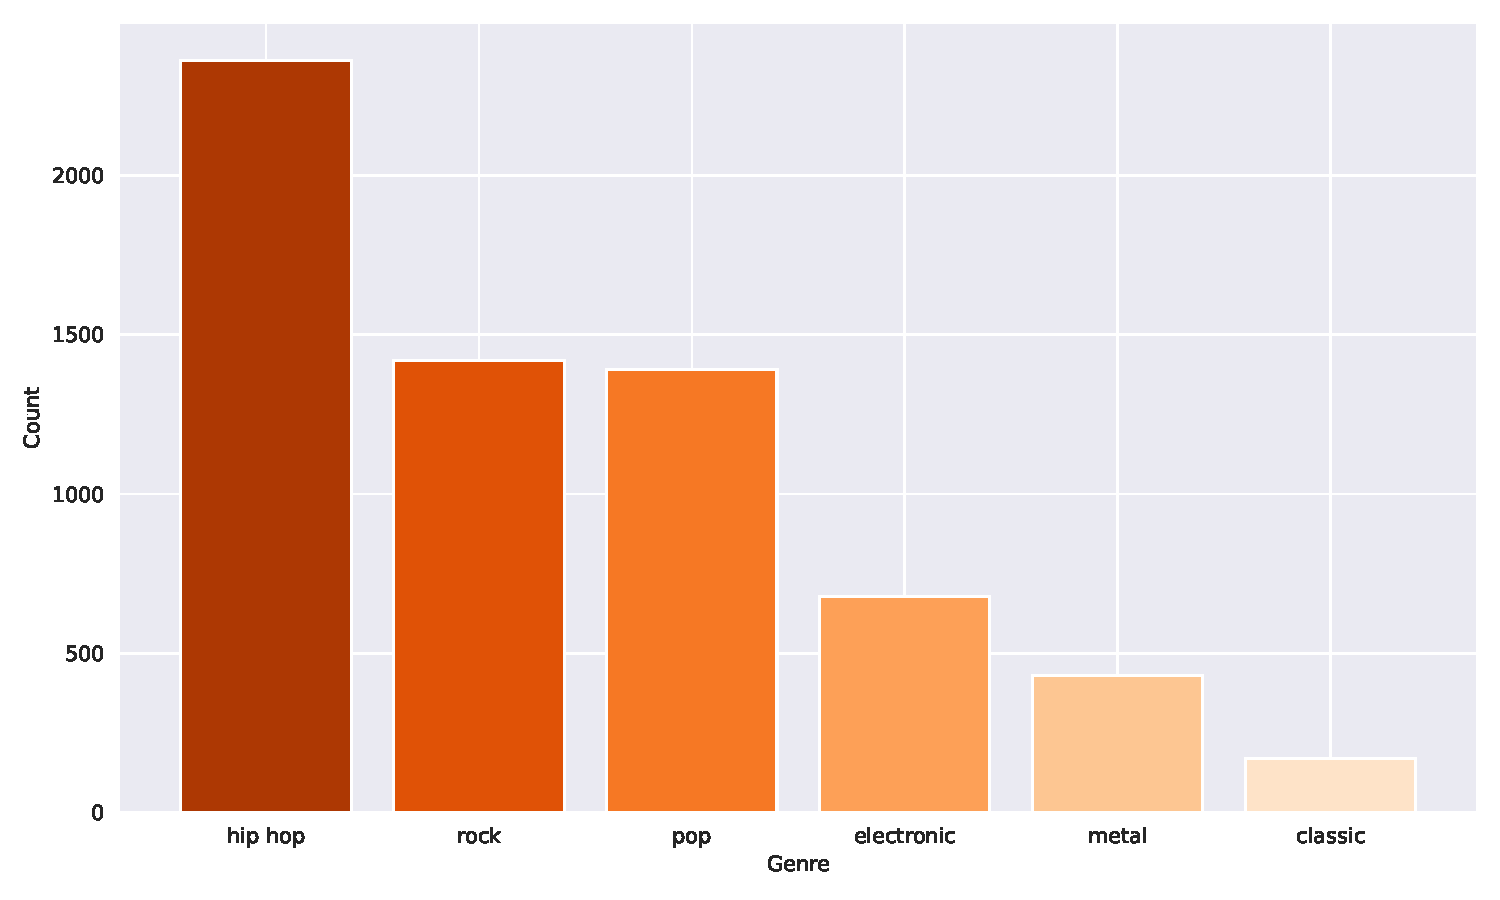
\includegraphics[scale=0.5]{figures/genre_hist_oranges.pdf}
  \caption{Class imbalance of the resulting dataset.}
  \label{fig:class-imbalance}
\end{figure}
\FloatBarrier
\noindent
Upon application of the preprocessing steps, the dataset is reduced to $6446$ entries.
Given the high class imbalance in our dataset, the use of weights could potentially help mitigate this imbalance. However, in our specific case, we found that weighting did not improve model performance. Therefore, we decided not to use weighting in our final modelling approach.
To enhance the sample size for the under-represented classes, synthesizing new entries could be a potential strategy for future work.
After this step, the dataset is divided into a training-, test- and validation-set, with each containing $\SI{80}{\percent}$, $\SI{16}{\percent}$ and $\SI{4}{\percent}$
of the data respectively.
\section{The dense Neural Network Model}
% a. Implementierung: Beschreibung der Implementierung des neuronalen Netzwerks.
% b. Ergebnisse: Wie hat das neuronale Netzwerk im Vergleich zu den anderen Methoden abgeschnitten?
% c. Diskussion: Warum hat das neuronale Netzwerk besser oder schlechter abgeschnitten?
\subsection{Architecture and Implementation}
The sequential dense neural network employed to solve this task is composed of two hidden layers. Increasing the layer count further proved to result in no additional
performance gains. The same holds true for using more neurons per layer, suggesting both strategies may lead to over-fitting.
To combat over-fitting, we use dropouts between each dense layer as well as learning rate decay and early stopping.
The later also reduces the needed computation time and annealing the learning rate increases the convergence speed. The output layer uses the activation function softmax,
as it can be used to return a probability distribution for the classes. To measure the performance and loss, we use the accuracy and the categorical crossentropy respectively.
The network architecture and the output shape of each layer can be seen in figure~\ref{fig:nn_layers}.
\begin{figure}[H]
    \centering
    \begin{minipage}{0.49\textwidth}
        \centering
        \footnotesize
        \begin{tabular}{l c}
            \toprule
            Parameter & Value \\
            \midrule
            Activation Function     & LeakyReLU \\
            Batch Size              & $512$     \\
            Dropout Rate            & $0.4$     \\
            Early Stopping Patience & $20$      \\
            Epochs                  & $60$      \\
            Neurons Layer (1)       & $256$     \\
            Neurons Layer (2)       & $512$     \\
            Neurons Layer (3)       & $512$     \\
            Number of hidden Layers & $2$       \\
            Optimizer               & Nadam     \\
            Reduce LR Factor        & $0.1$     \\
            Min. LR Rate            & $0.0$     \\
            Reduce LR Patience      & $5$       \\
            Output Function         & Softmax   \\
            % Weight Constraint       & $10$      \\
            \bottomrule
        \end{tabular}
        % \caption{All parameters of the best performing model.}
        \label{tab:my_label_for_table}
    \end{minipage}
    \begin{minipage}{0.49\textwidth}
        \centering
        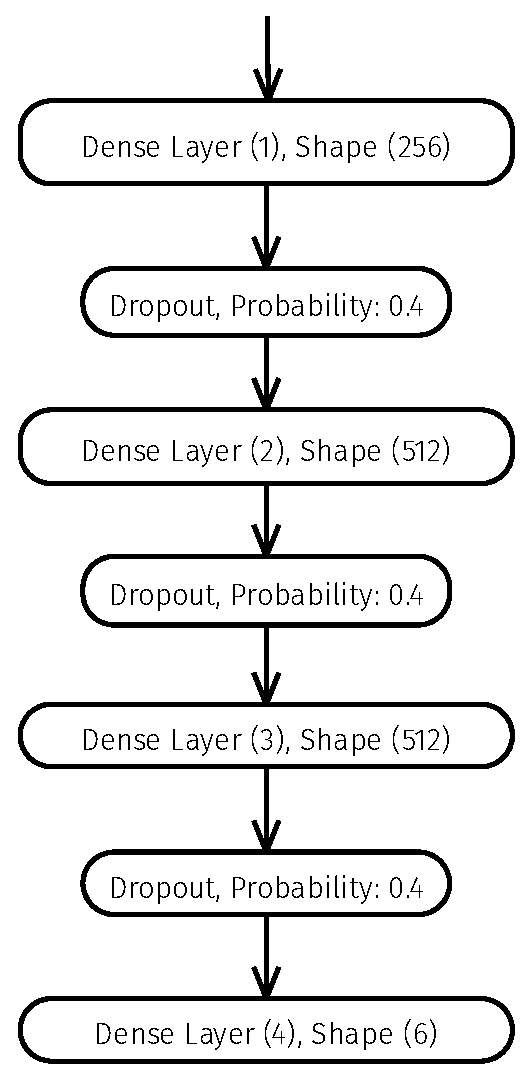
\includegraphics[width=0.5\textwidth]{figures/Network.pdf}
        % \caption{Overview of the neural networks' layers and parameters.}
        % \label{fig:nn_layers}
        \normalsize
    \end{minipage}\hfill
  \caption{Overview of the neural networks' layers and parameters.}
  \label{fig:nn_layers}
\end{figure}
\noindent
We implement the model using \texttt{tensorflow}~\cite{tensorflow} and \texttt{keras}~\cite{keras}.
\subsection{Hyperparameter Optimization}
The exact parameters given in figure~\ref{fig:nn_layers} are the result of performing a hyperparameter optimization. For this, we carry out a
grid search~\cite{gridsearch}, implemented with \texttt{GridSearchCV} from \texttt{Scikit-Learn}~\cite{scikit-learn}, as it supports parallel computing.
We use $3$-fold cross-validation  to mitigate overfitting and to make efficient use of the finite data.
To be able to optimize a model created by \texttt{keras} with \texttt{Scikit-Learn} functions, we use \texttt{SciKeras}~\cite{scikeras}. As we were limited in time and
computational resources, only a subset of the parameter space has been explored; for most parameters, we tried between two and six values, but
not all combinations of them. Still, $2033$ models were tested, with \ref{fig:nn_layers} resulting in the highest performance. All tested models and their performance can be
seen here\footnote{\url{https://github.com/Henry-Kr15/TheGenreFactor/blob/main/HPO-data/HPO_combined.csv}}.
Selecting the best model is a trade-off between accuracy on the training set and overfitting, which results in lower performance on the validation set. Because of the limited
size of the validation set (as it comprises of only $\SI{4}{\percent}$ of the data), relying on validation accuracy alone could prove inconsistent. We try to manually alter
this trade-off to achieve higher generalisation than otherwise possible. For this, we combine the validation accuracy and training accuracy into a new metric which we call
delta accuracy by taking the difference of the two. Then we calculate a score based on the delta and validation accuracy as follows:
\begin{equation}
	\text{score} = \frac{1}{2} \cdot (w_{1} \cdot (1 - \text{acc}_{\text{delta}}) + w_{2} \cdot \text{acc}_{\text{test}}).
  \label{eqn:score}
\end{equation}
The score minimizes $\text{acc}_{\text{delta}}$ whilst maximizing $\text{acc}_{\text{test}}$. Using the weights $w_{1}$ and $w_{2}$, the importance of each value can be specified.
All models can be seen in figure~\ref{fig:HPO_scatter}. With $w_{1}=0.5$ and $w_{2}=1$ the model marked red has the best score.
\begin{figure}[H]
  \centering
  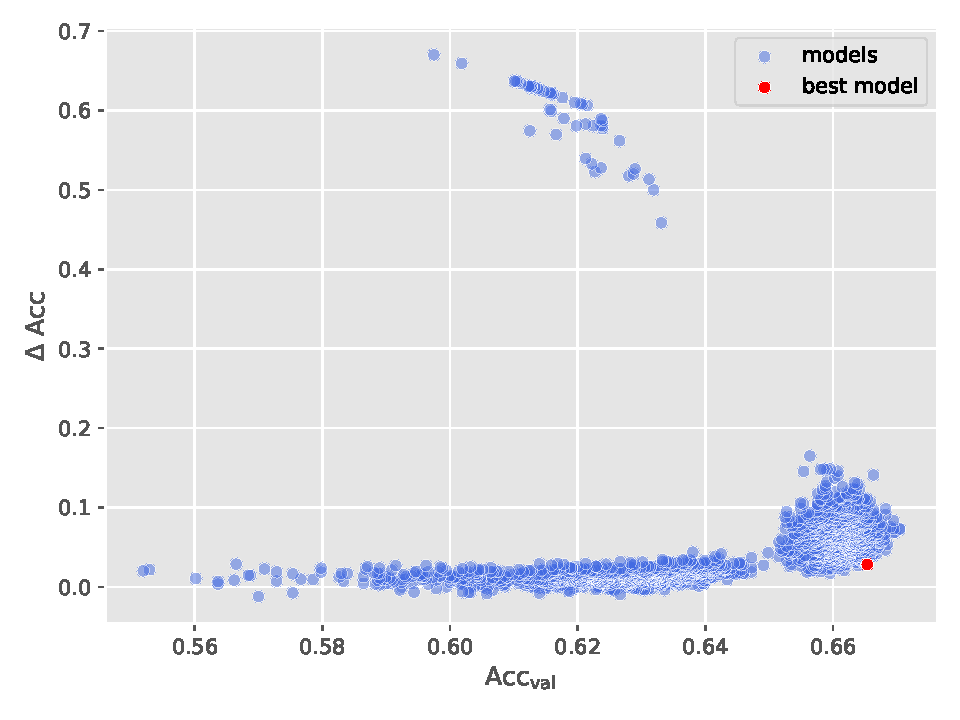
\includegraphics[scale=0.56]{figures/NN/HPO_scatter.pdf}
  \caption{Comparison of training and delta accuracy for all models.}
  \label{fig:HPO_scatter}
\end{figure}
\subsection{Performance and Results}
The model achieves $\SI{64.43}{\percent}$ accuracy on the test data set. Accuracy and loss are shown in figure~\ref{fig:nn_acc} and figure~\ref{fig:nn_loss} respectively.
\begin{figure}[H]
  \centering
  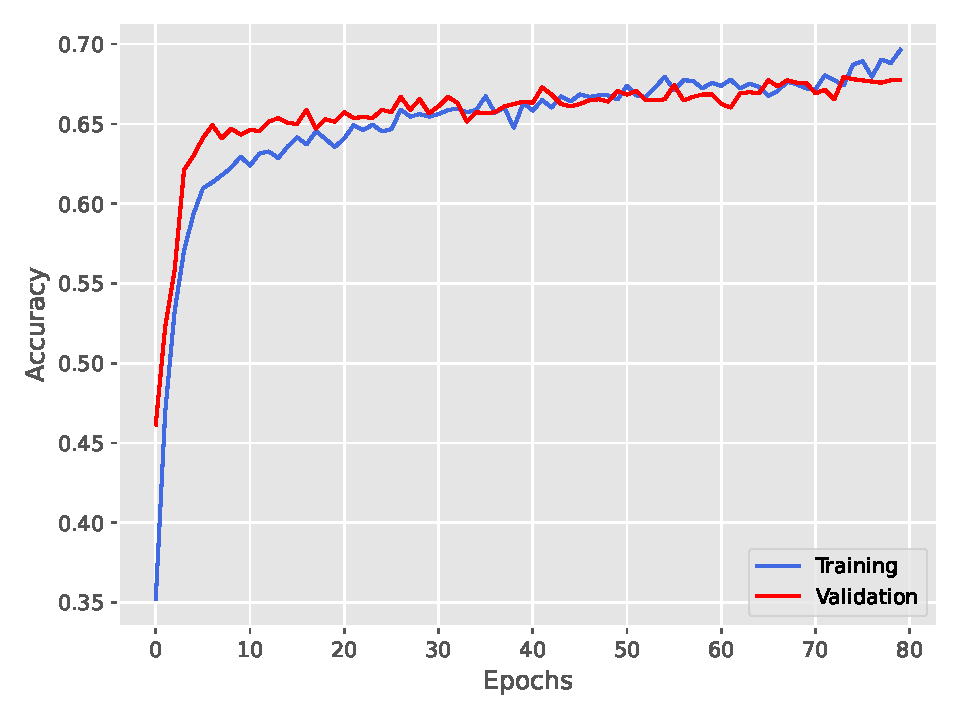
\includegraphics[scale=0.56]{figures/NN/Acc.pdf}
  \caption{Plot of the accuracy of the neural network on the training and validation dataset.}
  \label{fig:nn_acc}
\end{figure}
\begin{figure}[ht]
  \centering
  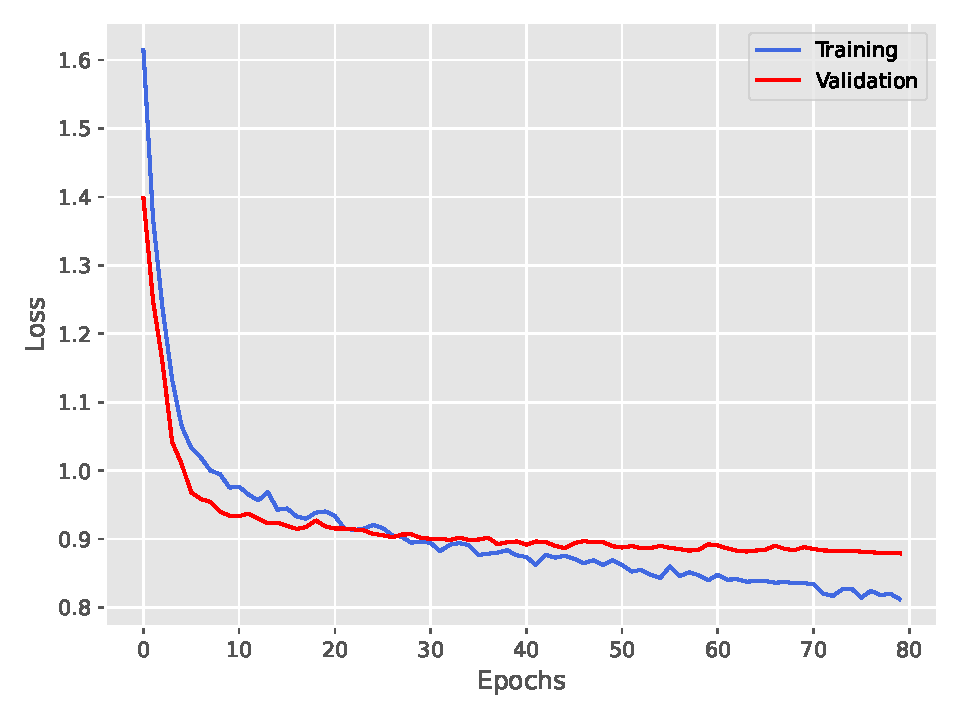
\includegraphics[scale=0.56]{figures/NN/Loss.pdf}
  \caption{Plot of the loss curve of the neural network on the training and validation dataset.}
  \label{fig:nn_loss}
\end{figure}
\noindent
The accuracy curve shows a satisfactory trend, indicating that the model is performing well on both the training and validation datasets. The loss curve however
shows a slight indication of overfitting after approximately $40$ epochs.
The confusion matrix can be seen in figure~\ref{fig:nn_confusion}.
\begin{figure}[H]
  \centering
  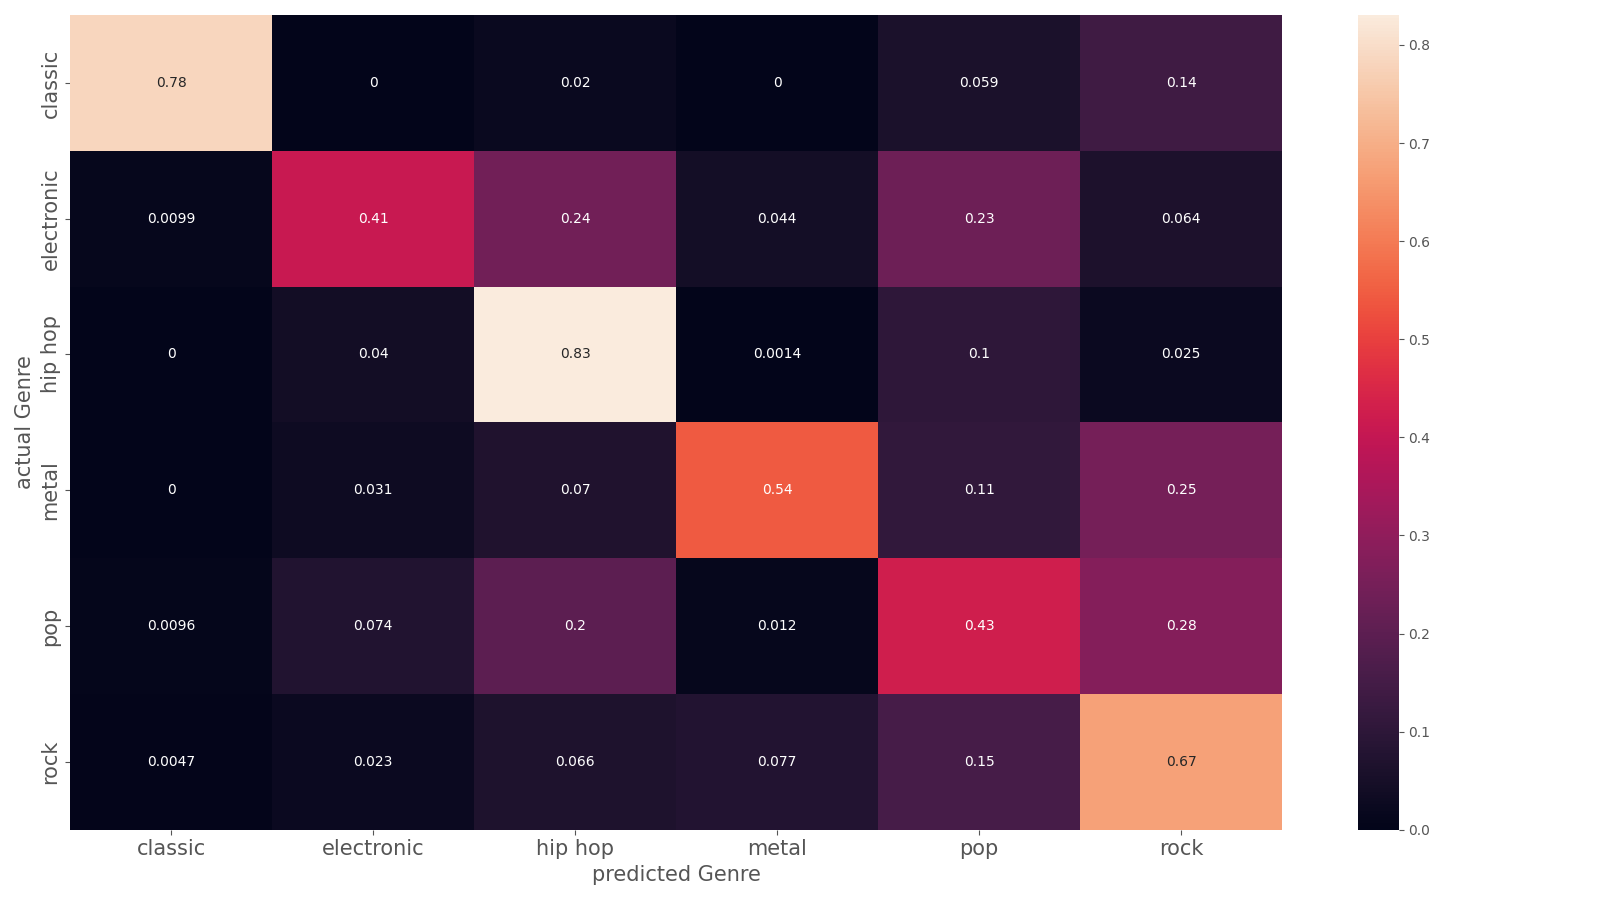
\includegraphics[scale=0.4]{figures/NN/confusion_matrix_nn.png}
  \caption{Confusion matrix of the neural network on the test dataset.}
  \label{fig:nn_confusion}
\end{figure}
\noindent
The confusion matrix shows, that although the models performance is for the most part adequate, problems arise for genres which consist of a broader spectrum with less clear
defined characteristics, such as pop or electronic. Differentiating rock from metal and pop seems to be more difficult as well; this conforms to the areas where humans would
also struggle. Astonishingly, the neural network performs the best for classic, which had the lowest sample size of any genre.
The precision-recall curve, depicted in figure~\ref{fig:pr_curve_nn}, shows a comparable result.
\begin{figure}[H]
  \centering
  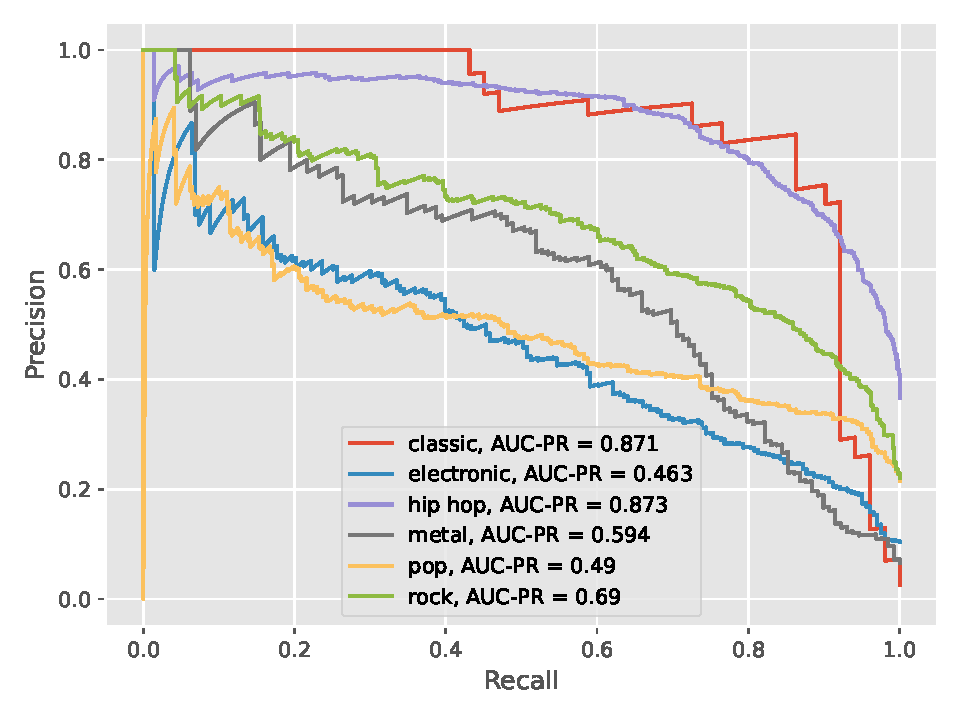
\includegraphics[scale=0.56]{figures/NN/PR_curve_genres.pdf}
  \caption{Precision-recall curve for each genre on the test dataset.}
  \label{fig:pr_curve_nn}
\end{figure}
\noindent
Classic and hip hop seem to get differentiated well, while pop and electronic show suboptimal performance.

\section{Alternative Approaches to the Problem}
% a. Leistung von Knn: Wie hat das Knn-Modell abgeschnitten?
% b. Leistung von SVM: Wie hat das SVM-Modell abgeschnitten?
% c. Diskussion: Vergleich der beiden Modelle auf der Grundlage ihrer Ergebnisse.
\subsection{Exploration of alternative Methods: K-Nearest Neighbours}
In addition to the neural network, we also explored other machine learning methods for comparison. One such method is the K-Nearest Neighbors (KNN) algorithm, a simpler
method which can be used for classification as well. This section provides an overview of our implementation and evaluation of the KNN approach.
\subsection{Exploration of alternative Methods: Support Vector Machines}
Another alternative method we investigated is the Support Vector Machine (SVM) approach. Through combining multiple SVMs, using them for classification tasks is possible.
This section discusses our implementation and performance of the SVM method in the context of our project.
\section{Discussion and Insights}
% a. Allgemeine Diskussion: Zusammenfassung der Erkenntnisse aus dem Projekt.
% b. Schlussfolgerungen: Was sind die endgültigen Schlussfolgerungen aus dem Projekt?
% c. Zukünftige Arbeiten: Gibt es Bereiche, in denen weitere Arbeit durchgeführt werden könnte?
\printbibliography

\end{document}
